% 2020年北京高考数学第16题：正方体与平面截面
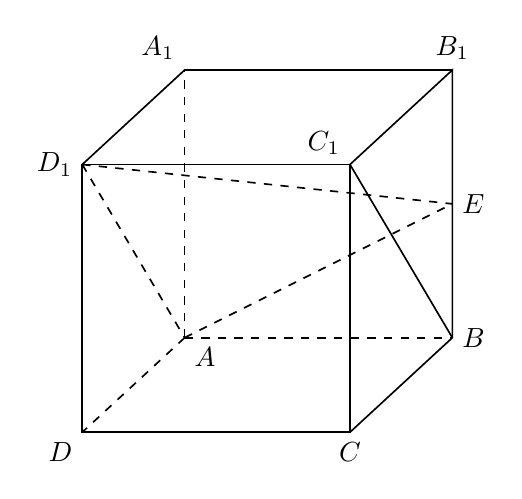
\begin{tikzpicture}[>=stealth,line width=0.6pt,font=\normalsize]
  \coordinate (A) at (0,0);
  \coordinate (D) at (-1.3,-1.2);
  \coordinate (B) at (3.4,0);
  \coordinate (C) at (2.1,-1.2);
  \coordinate (A1) at (0,3.4);
  \coordinate (D1) at (-1.3,2.2);
  \coordinate (B1) at (3.4,3.4);
  \coordinate (C1) at (2.1,2.2);
  \coordinate (E) at (3.4,1.7);

  % 实线可见边
  \draw (D) -- (D1) -- (C1) -- (C) -- cycle;
  \draw (C1) -- (B1) -- (B) -- (C);
  \draw (D1) -- (A1) -- (B1);
  \draw (B) -- (C1);

  % 虚线不可见边与截面线
  \draw[dashed] (A) -- (A1);
  \draw[dashed] (A) -- (D);
  \draw[dashed] (A) -- (B);
  \draw[dashed] (D1) -- (A);
  \draw[dashed] (A) -- (E);
  \draw[dashed] (D1) -- (E);

  % 顶点标注
  \node[below right] at (A) {$A$};
  \node[right] at (B) {$B$};
  \node[below] at (C) {$C$};
  \node[below left] at (D) {$D$};
  \node[above left] at (A1) {$A_1$};
  \node[above] at (B1) {$B_1$};
  \node[above left] at (C1) {$C_1$};
  \node[left] at (D1) {$D_1$};
  \node[right] at (E) {$E$};
\end{tikzpicture}
